\section{Experiments}
\label{sec:results}

\subsection{Robustness and its zero-shot transfer}
\label{sec:robustness}

\Cref{tab:accuracy} reports clean and corrupted accuracy. GRPO is strongest on every
backbone, raising corrupted accuracy over the base model by $7.6$ (Qwen3-VL-4B), $6.6$
(InternVL3.5-4B) and $5.2$ points (Gemma-3-4B), and also raising clean accuracy; on
Qwen3-VL-4B its largest gains are on GQA-C ($+10.2$) and VQAv2-C ($+9.5$, per-benchmark
numbers in \cref{tab:supp_full_bench}). RKL improves corrupted accuracy by $2.1$--$5.3$ points and
holds clean accuracy flat on Qwen3-VL-4B. The gains transfer to corruption types never seen
in training (\cref{fig:per-corruption}): on the $11$ unseen types GRPO gains $8.7$ points on
average, against $8.2$ on the $8$ seen types, and RKL gains $1.9$ against $2.2$. The only
negative point estimate, RKL on speckle noise ($-1.7 \pm 2.1$), is within noise. Robust
fine-tuning therefore does what it is meant to do, and it generalizes.

\begin{figure}[t]
  \centering
  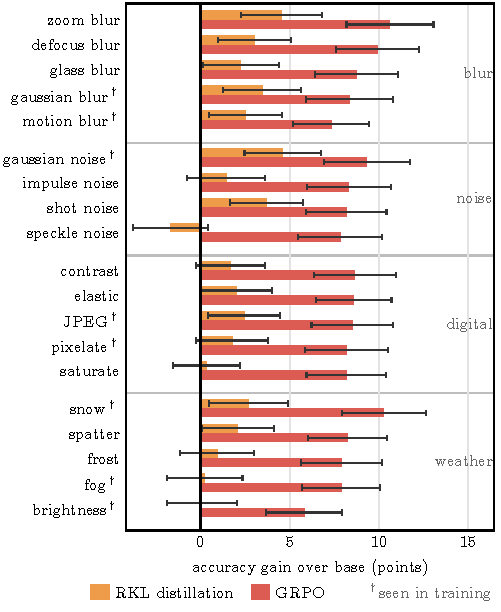
\includegraphics[width=\columnwidth]{figures/per_corruption_gain.pdf}
  \caption{\textbf{Both recipes' gains transfer to corruption types never seen in training.}
  Accuracy gain of Qwen3-VL-4B over its base model per corruption type, pooled over the
  TextVQA-C, GQA-C and VQAv2-C questions of each type (all five severities,
  ${\sim}1{,}190$ questions per type). Error bars: 95\% CI of the paired difference.
  $\dagger$: type seen in training.}
  % src: docs/iclr2027/figures/per_corruption/per_corruption_gain.csv
  % (seen/unseen means in Sec. 5.2 computed from the same file)
  \label{fig:per-corruption}
\end{figure}

\begin{table}[t]
\centering
\caption{\textbf{Robust fine-tuning raises clean and corrupted accuracy on every backbone,
and GRPO gains most.}}
% src: outputs/eval/full-*/results.jsonl (vLLM rows); outputs/steer_full/*/eval (steering);
%      probe rows: /gscratch/dsikdar/tmp_scripts/probe_table3_strict_tau.py (tau_p = 2)
\label{tab:accuracy}
\small
\setlength{\tabcolsep}{4pt}
\begin{tabular}{lcc}
\toprule
Method & Corrupted $\uparrow$ & Clean $\uparrow$ \\
\midrule
\multicolumn{3}{l}{\textit{Qwen3-VL-4B, full fine-tuning}} \\
Base                                          & 64.26 & 72.09 \\
RKL (8B teacher)                              & 66.38 & 72.15 \\
\quad + unanswerable mix (10\%)               & 65.71 & 71.71 \\
\quad + steering, image-contrast, gated$^\ast$  & 66.57 & 72.62 \\
\quad + steering, image-contrast, always$^\ast$ & 65.59 & 71.69 \\
\quad + LATCH$^\ast$                          & 66.42 & 72.34 \\
GRPO                                          & 71.84 & 79.01 \\
\quad + unanswerable mix (10\%)               & 71.59 & 78.48 \\
\quad + steering, no-image, gated$^\ast$      & 71.96 & 79.01 \\
\quad + steering, no-image, always$^\ast$     & 71.72 & 78.80 \\
\quad + LATCH$^\ast$                          & 71.43 & 78.73 \\
\midrule
\multicolumn{3}{l}{\textit{InternVL3.5-4B, full fine-tuning$^\ddagger$}} \\
Base                                          & 61.35 & 70.04 \\
RKL (14B teacher)                             & 66.64 & 74.05 \\
\quad + unanswerable mix (10\%)               & 66.45 & 74.05 \\
\quad + steering, image-contrast, gated$^\ast$  & 66.86 & 74.13 \\
\quad + steering, image-contrast, always$^\ast$ & 66.55 & 74.16 \\
\quad + LATCH$^\ast$                          & 66.45 & 74.01 \\
GRPO                                          & 68.00 & 76.45 \\
\quad + unanswerable mix (10\%)               & 67.57 & 75.83 \\
\quad + steering, no-image, gated$^\ast$      & 68.03 & 76.46 \\
\quad + steering, no-image, always$^\ast$     & 67.97 & 76.61 \\
\quad + LATCH$^\ast$                          & 67.95 & 76.47 \\
\midrule
\multicolumn{3}{l}{\textit{Gemma-3-4B, full fine-tuning$^\S$}} \\
Base                                          & 55.44 & 62.76 \\
RKL (12B teacher)                             & 58.94 & 65.79 \\
\quad + unanswerable mix (10\%)               & 56.37 & 63.08 \\
\quad + steering, image-contrast, gated$^\ast$  & 59.01 & 65.71 \\
\quad + steering, image-contrast, always$^\ast$ & 59.10 & 65.39 \\
\quad + steering, no-image, gated$^\ast$      & 59.09 & 65.95 \\
\quad + steering, no-image, always$^\ast$     & 58.09 & 64.32 \\
\quad + LATCH$^\ast$                          & 58.58 & 65.22 \\
GRPO                                          & 60.65 & 66.68 \\
\quad + unanswerable mix (10\%)               & 60.71 & 67.66 \\
\quad + steering, image-contrast, gated$^\ast$  & 60.40 & 66.81 \\
\quad + steering, image-contrast, always$^\ast$ & 60.16 & 66.57 \\
\quad + steering, no-image, gated$^\ast$      & 60.56 & 66.66 \\
\quad + steering, no-image, always$^\ast$     & 60.70 & 66.90 \\
\quad + LATCH$^\ast$                          & 59.38 & 66.13 \\
\bottomrule
\end{tabular}
\end{table}


\begin{table*}[t]
\centering
\caption{\textbf{Robust fine-tuning lowers correct refusals on every backbone;
LATCH recovers $16$--$39$ points of them while adding at most $2.8$ points of unnecessary
refusals.} }
% src: outputs/eval/full-*/results.jsonl, outputs/eval/{base4b-sys,fullft_*}-extra (vLLM rows);
%      outputs/steer_full/*/eval (steering); outputs/probe_switch/*/report.json (probe, tau_p = 2)
\label{tab:refusal}
\small
\begin{tabular}{lccccc}
\toprule
& \multicolumn{4}{c}{VizWiz} & No-image \\
\cmidrule(lr){2-5}\cmidrule(lr){6-6}
Method & Ans.\ acc.\ $\uparrow$ & UR $\downarrow$ & CR $\uparrow$ & Unans.\ acc.\ $\uparrow$
       & refusals $\uparrow$ \\
\midrule
\multicolumn{6}{l}{\textit{Qwen3-VL-4B, full fine-tuning}} \\
Base                                          & 40.6 & 12.8 & 71.6 & 76.0 & 52.0 \\
RKL (8B teacher)                              & 50.4 &  8.4 & 49.6 & 56.5 &  1.0 \\
\quad + unanswerable mix (10\%)               & 48.3 & 13.3 & 61.7 & 66.9 &  2.2 \\
\quad + steering, image-contrast, gated$^\ast$  & 50.4 & 11.1 & 57.5 & 64.1 &  1.6 \\
\quad + steering, image-contrast, always$^\ast$ & 47.1 & 18.0 & 69.0 & 73.2 &  3.0 \\
\quad + LATCH$^\ast$                          & 50.3 & 10.0 & 65.4 & 71.6 & 18.6 \\
GRPO                                          & 60.9 &  3.2 & 44.9 & 60.3 &  0.5 \\
\quad + unanswerable mix (10\%)               & 60.9 &  6.1 & 56.9 & 69.7 & 31.4 \\
\quad + steering, no-image, gated$^\ast$      & 60.8 &  5.4 & 51.2 & 65.9 &  0.4 \\
\quad + steering, no-image, always$^\ast$     & 57.3 & 14.5 & 70.7 & 81.7 &  0.4 \\
\quad + LATCH$^\ast$                          & 60.3 &  5.4 & 61.2 & 73.0 & 31.6 \\
\midrule
\multicolumn{6}{l}{\textit{InternVL3.5-4B, full fine-tuning$^\ddagger$}} \\
Base                                          & 41.7 & 11.2 & 58.6 & 64.5 &  2.0 \\
RKL (14B teacher)                             & 47.6 &  6.9 & 34.0 & 42.0 &  0.1 \\
\quad + unanswerable mix (10\%)               & 46.6 & 14.6 & 62.7 & 67.2 &  2.0 \\
\quad + steering, image-contrast, gated$^\ast$  & 46.7 &  7.2 & 35.2 & 42.9 &  0.1 \\
\quad + steering, image-contrast, always$^\ast$ & 47.0 &  7.7 & 37.9 & 44.9 &  0.1 \\
\quad + LATCH$^\ast$                          & 46.9 &  8.6 & 60.0 & 65.9 & 11.0 \\
GRPO                                          & 53.6 &  2.5 & 25.9 & 39.0 &  0.0 \\
\quad + unanswerable mix (10\%)               & 52.7 &  3.6 & 31.2 & 43.7 &  0.8 \\
\quad + steering, no-image, gated$^\ast$      & 53.3 &  2.7 & 25.8 & 39.0 &  0.0 \\
\quad + steering, no-image, always$^\ast$     & 52.6 &  3.2 & 29.5 & 41.4 &  0.1 \\
\quad + LATCH$^\ast$                          & 52.2 &  5.4 & 56.6 & 66.6 &  3.9 \\
\midrule
\multicolumn{6}{l}{\textit{Gemma-3-4B, full fine-tuning$^\S$}} \\
Base                                          & 48.1 &  5.0 & 28.2 & 34.4 &  2.1 \\
RKL (12B teacher)                             & 53.1 &  2.0 & 11.8 & 22.5 &  0.0 \\
\quad + unanswerable mix (10\%)               & 51.7 &  4.2 & 25.8 & 35.0 &  1.4 \\
\quad + steering, image-contrast, gated$^\ast$  & 52.6 &  2.3 & 11.9 & 22.6 &  0.0 \\
\quad + steering, image-contrast, always$^\ast$ & 53.2 &  2.2 & 12.4 & 22.4 &  0.1 \\
\quad + steering, no-image, gated$^\ast$      & 52.0 &  4.4 & 21.1 & 31.1 &  0.3 \\
\quad + steering, no-image, always$^\ast$     & 48.9 &  6.1 & 27.8 & 36.0 &  3.4 \\
\quad + LATCH$^\ast$                          & 53.0 &  4.5 & 50.2 & 58.6 & 61.4 \\
GRPO                                          & 48.8 &  0.4 & 10.9 & 24.5 &  0.0 \\
\quad + unanswerable mix (10\%)               & 50.7 &  1.4 & 14.7 & 28.7 &  0.0 \\
\quad + steering, image-contrast, gated$^\ast$  & 48.5 &  0.5 & 10.9 & 24.5 &  0.0 \\
\quad + steering, image-contrast, always$^\ast$ & 48.2 &  0.5 & 10.0 & 23.9 &  0.0 \\
\quad + steering, no-image, gated$^\ast$      & 48.7 &  0.6 & 12.1 & 26.1 &  0.0 \\
\quad + steering, no-image, always$^\ast$     & 48.5 &  1.0 & 15.2 & 28.4 &  0.0 \\
\quad + LATCH$^\ast$                          & 48.8 &  2.9 & 43.2 & 54.3 & 92.6 \\
\bottomrule
\end{tabular}
\end{table*}


\subsection{The silent abstention regression}
\label{sec:regression}

% Review note: the sentence "the most accurate model is the worst abstainer" holds on CR
% (GRPO < RKL on all three backbones) but not on the unanswerable accuracy quoted here
% (GRPO 60.3 > RKL 56.5). The no-image accuracies below are in no table.
The same training degrades abstention, first on real degradation and then, more sharply,
on missing images. VizWiz unanswerable accuracy (\cref{tab:refusal}) falls from $76.0$
(base) to $60.3$ (GRPO) and $56.5$ (RKL) for the Qwen backbone. With the image withheld, base accuracy sits near
the floor ($1.9$--$14.5$), but the fine-tuned models answer anyway, GRPO reaching $46.0$ on
VQAv2 and $36.3$ on GQA. We see a similar kind of pattern for the other backbones as well where the fine tuned model regressed when it comes to answering questions when the answer is not there. All this scores are address in \cref{tab:refusal}

\subsection{RQ1: Is answerability erased, or only suppressed?}
\label{sec:rq1}

% probe_answerability.py analyze: L2 strength defaults to 0.01 (or 5-fold CV with --cv-*);
% LATCH uses 0.1. State which one the Tab. 5 run used.
The probe of \cref{eq:probe}, fitted at every layer on the VizWiz-train pool $\mathcal{C}$
(\cref{sec:setup}), separates answerable from unanswerable VizWiz-val questions at $\mathrm{AUROC}\approx0.93$ in the base,
RKL and GRPO models of Qwen3-VL-4B, far above the shuffled-label control
(\cref{tab:probe}): fine-tuning does not erase the representation of answerability. Among
the unanswerable questions the fine-tuned models wrongly answered, the probe still flags
$76$--$77\%$ as unanswerable ($711$ items for RKL, $765$ for GRPO). The models internally
``know'' these inputs are unanswerable, yet answer them. The lone exception is
image-missingness: with the image withheld (\cref{tab:probenoimg}) the flag rate collapses
for RKL (GQA $68\% \rightarrow 31\%$), so RKL has partly lost its sense that the image is
gone, while GRPO keeps it. The failure is thus one of behavior, not knowledge.

\begin{table}[tb]
\centering
\small
\caption{\textbf{Answerability stays linearly decodable after fine-tuning} (Qwen3-VL-4B,
VizWiz val). Shuffled: AUROC of the same probe trained on shuffled labels. The best layer is
chosen by VizWiz-val AUROC, i.e.\ on the evaluation split.}
\label{tab:probe}
\begin{tabular}{@{}lccc@{}}
\toprule
Model & Best layer & Probe AUROC & Shuffled \\
\midrule
Base & 23 & 0.931 & 0.48 \\
RKL  & 24 & 0.927 & 0.52 \\
GRPO & 23 & 0.930 & 0.50 \\
\bottomrule
\end{tabular}
\end{table}

\begin{table}[tb]
\centering
\small
\caption{\textbf{RKL loses much of its sense that the image is missing.} Share (\%) of
questions asked without their image that the probe flags as unanswerable (Qwen3-VL-4B).}
\label{tab:probenoimg}
\begin{tabular}{@{}lcccc@{}}
\toprule
Model & GQA & VQAv2 & TextVQA & VizWiz \\
\midrule
Base & 68 & 75 & 98 & 100 \\
RKL  & 31 & 38 & 94 & 99 \\
GRPO & 56 & 64 & 98 & 100 \\
\bottomrule
\end{tabular}
\end{table}

\subsection{RQ2: Do the two recipes fail the same way?}
\label{sec:rq2}

They fail oppositely (\cref{tab:transplant}). Handed the base model's ``can't-tell''
chain by the reasoning transplant (\cref{sec:method-diagnose}), RKL refuses $98.4\%$ of the
time, so its failure is that its own reasoning never reaches that chain. In this case, we look only at the first word $\pi_\theta$ would write after <answer> and if its most likely word is a refusal (e.g., "unanswerable" or "cannot"), we count it as a refusal. Consistently, RKL's responses on these items are far longer
than the base model's or GRPO's: on the unanswerable set its median response is $98$
tokens against $71$ (base) and $77$ (GRPO), and on the subset where it runs long the gap
widens to $341.5$ tokens against ${\sim}109$ for both others on the same questions
---the signature of an unsure, high-entropy chain that talks itself into
an answer, often running to the $768$-token limit. GRPO, given the identical chain, still
answers $91.8\%$ of the time: its reasoning is sound, but it has learned an answer-level
shortcut, committing to a definitive answer no matter what the chain concludes, because the
exact-match reward always paid off for answering. In short, RKL cannot reason its way to
unanswerability; GRPO reasons there but will not act on it.

\begin{table}[tb]
\centering
\small
\caption{\textbf{RKL fails on the reasoning side, GRPO on the answer side.} Reasoning
transplant (\cref{sec:method-diagnose}, Qwen3-VL-4B): share of items the fine-tuned model
refuses when given the base model's ``can't-tell'' chain.}
\label{tab:transplant}
\begin{tabular}{@{}lcc@{}}
\toprule
Model & Items & Refuses w/ ``can't-tell'' chain \\
\midrule
RKL  & 308 & 98.4\% \\
GRPO & 389 & 8.2\% \\
\bottomrule
\end{tabular}
\end{table}

\subsection{RQ3: Recovering abstention without losing the gains}
\label{sec:rq3}

% Review note: the LATCH numbers at tau_p = 1 (73--77%, 10--14%, at most 1.2 points),
% the 31--63% / 41--58% ranges, "11--51%" and the RKL no-image steering row (88.6/45.4) are
% not in Tabs. 3-4; the tables appear to report tau_p = 0.

On every fine-tuned model, LATCH restores abstention best. It refuses
when the probe's predicted probability that a question is unanswerable exceeds a cutoff
$p_{\mathrm{c}}$; \cref{tab:accuracy,tab:refusal} use $p_{\mathrm{c}} = 0.88$. At this
cutoff it raises correct refusals on VizWiz from $11$--$50\%$ to $43$--$65\%$
($16$--$39$ points) while adding only $1.5$--$2.8$ points of unnecessary refusals, and it
costs at most $0.4$ points of corrupted accuracy ($1.3$ on Gemma-3-4B GRPO) and at most
$1.4$ points of answerable accuracy. The unanswerable mix and steering approach or exceed
its correct refusals only on Qwen3-VL-4B and InternVL3.5-4B RKL, and only at $13$--$18\%$
unnecessary refusals. LATCH is also the only inference-time remedy that consistently
flags a missing image ($4$--$93\%$ of no-image questions, against at most $3.4\%$ for
steering). Lowering the cutoff trades accuracy for recall: $p_{\mathrm{c}} = 0.73$ reaches
$62$--$77\%$ correct refusals at $8$--$14\%$ unnecessary refusals, and $p_{\mathrm{c}} = 0.5$
reaches $81$--$88\%$ at $17$--$23\%$, at a cost of $0.9$--$8.9$ corrupted points.


The reason is that robust fine-tuning suppresses abstention in the model's output but
leaves answerability linearly decodable from its residual stream. LATCH reads this
signal once, before generation, and leaves the answer untouched when it does not fire, so
the robustness gained on answerable inputs is preserved, and a single threshold sets the
trade-off ($\tau_{\mathrm{p}} = 0$ raises correct refusals to $85$--$88\%$ at roughly twice
the unnecessary refusals).

Steering reads the same representation but acts through one fixed direction added at every
decoding step, so triggering refusals and preserving answers conflict. On Qwen3-VL-4B RKL,
always-on no-image steering reaches $88.6\%$ correct refusals but refuses $45.4\%$ of
answerable questions and loses $8.9$ points of accuracy. Steering is also fragile across
models: the best direction differs between models, and on Gemma-3-4B no configuration
raises correct refusals by more than $7$ points, whereas LATCH, unchanged, lifts
them from $11$--$13\%$ to $81$--$82\%$.

Retraining helps without test-time machinery, but it needs a full training run and
recovers less, because its unanswerable examples are GQA questions on destroyed images,
while real VizWiz questions are unanswerable for subtler reasons (blur, framing, an object
out of view). It also barely teaches refusal on a missing image ($0.8$--$2.2\%$, except
$31\%$ for Qwen3-VL-4B GRPO). RKL absorbs the mix better than GRPO: the student is pulled
toward a teacher that refuses readily on destroyed images (RKL gains $13$--$29$ points),
whereas GRPO sees the label only through a sparse exact-match reward (InternVL3.5-4B GRPO
gains $5$ points).

Overall, abstention remains recoverable after robust fine-tuning, and the cheapest remedy
works best: one logistic regression on $1{,}901$ calibration questions, with no retraining
and no change to decoding.
% requires \usepackage{booktabs}
% ------------------------------------------------------------
\subsection{Paired evidence-removal test}
\label{sec:paired_results}
% ------------------------------------------------------------

\begin{table*}[t]
\centering\small
\setlength{\tabcolsep}{3.2pt}
\begin{tabular}{l cccc c cccc c cccc}
\toprule
& \multicolumn{4}{c}{Qwen3-VL-4B} && \multicolumn{4}{c}{InternVL3.5-4B} && \multicolumn{4}{c}{Gemma-3-4B} \\
\cmidrule{2-5}\cmidrule{7-10}\cmidrule{12-15}
Model & Orig. & Ctrl. & Rem.$\uparrow$ & Cons.$\uparrow$ && Orig. & Ctrl. & Rem.$\uparrow$ & Cons.$\uparrow$ && Orig. & Ctrl. & Rem.$\uparrow$ & Cons.$\uparrow$ \\
\midrule
Base                     & 87.0 & 86.5 & 50.6 & 45.3 && 90.0 & 90.0 & 35.7 & 33.1 && 78.8 & 78.6 & 16.0 & 13.9 \\
\midrule
GRPO                     & 92.3 & 92.1 & 24.8 & 23.7 && 91.7 & 91.9 & 15.4 & 15.0 && 77.4 & 77.4 &  9.4 &  8.1 \\
\quad + steering$^\dagger$ & 91.5 & 91.5 & 49.6 & 46.8 && 92.3 & 92.5 & 19.2 & 18.4 && 77.1 & 75.6 & 12.0 & 10.3 \\
\quad + probe switch$^\dagger$ & 91.5 & 92.1 & 39.3 & 37.4 && 91.0 & 91.2 & 21.8 & 20.3 && 76.1 & 76.5 & 14.5 & 11.8 \\
GRPO-10\%                & 91.7 & 91.2 & 22.2 & 21.2 && 90.8 & 91.2 &  6.6 &  6.2 && 77.4 & 75.6 &  4.7 &  4.3 \\

\midrule
RKL$^\ddagger$           & 87.0 & 85.9 & 41.7 & 37.2 && 87.8 & 88.0 & 28.0 & 25.0 && 81.4 & 79.9 & 12.2 & 11.3 \\
\quad + steering$^\dagger$ & 76.9 & 77.4 & 73.1 & 54.5 && 82.7 & 83.3 & 54.1 & 44.2 && 79.5 & 79.5 & 22.4 & 18.8 \\
\quad + probe switch$^\dagger$ & 87.6 & 84.8 & 44.9 & 39.1 && 87.4 & 88.0 & 35.3 & 31.0 && 80.6 & 80.3 & 23.1 & 19.2 \\
RKL-10\%$^\ddagger$      & 85.5 & 84.4 & 45.7 & 39.7 && 87.2 & 87.2 & 36.1 & 31.0 && 79.5 & 81.0 & 16.5 & 14.1 \\
\bottomrule
\end{tabular}
\caption{\textbf{TextVQA-Paired} ($n{=}468$, strict scoring). Orig./Ctrl.: accuracy on the
original and control images. Rem.: evidence-removed accuracy (abstention rate when the
answer is erased). Cons.: correct on original and control \emph{and} abstaining on the
removed image. -10\%: trained with $10\%$ destroyed images labeled \emph{unanswerable}.
$^\dagger$No-image steering ($\lambda{=}1$, layer $18$) and probe switch ($\tau{=}2$),
fixed from the VizWiz experiments; HuggingFace decoding, whose unsteered baseline is
within $1.1$ points of the row above. $^\ddagger$Gemma: exact full-vocabulary RKL.}
\label{tab:paired}
\end{table*}

Table~\ref{tab:paired} reproduces the VizWiz trade-off under a controlled edit. The edit
itself is harmless: original and control accuracy agree within $3$ points for every model,
and unsteered models refuse at most $3.6\%$ of controls. Fine-tuning roughly halves
evidence-removed accuracy on all backbones (GRPO: Qwen $50.6\rightarrow24.8$, InternVL
$35.7\rightarrow15.4$, Gemma $16.0\rightarrow9.4$) while original accuracy rises or stays
flat, so models guess rather than abstain when the evidence is gone. The cause is the
objective, not the corrupted data: RKL retains more abstention than GRPO on every backbone
($41.7$, $28.0$, $12.2$), and GRPO trained on \emph{clean} images abstains even less
($17.9$). Adding $10\%$ unanswerable images restores RKL to roughly base-model abstention
($45.7$, $36.1$, $16.5$) but lowers it further for GRPO ($22.2$, $6.6$, $4.7$). Both fixes
transfer: the probe switch adds $4$--$13$ points at $\leq0.7$ points of original accuracy,
and separates removed from control images as well as from originals (AUROC within $0.3$),
so it detects missing evidence rather than the edit; no-image steering returns Qwen GRPO
to base-model abstention ($49.6$) at negligible cost, and gives the largest gains on RKL
($73.1$ Qwen, $54.1$ InternVL) at a cost of $5$--$11$ accuracy points. Neither fix helps
much on Gemma, whose base model abstains on only $16\%$ of removed images.
% requires \usepackage{booktabs,graphicx}
% ------------------------------------------------------------
\subsection{Is corrupted training data the cause?}
\label{sec:clean_grpo}
% ------------------------------------------------------------

\begin{table}[t]
\centering
\resizebox{\columnwidth}{!}{%
\begin{tabular}{l ccc cccc cc}
\toprule
& \multicolumn{3}{c}{Accuracy} & \multicolumn{4}{c}{VizWiz} & \multicolumn{2}{c}{Abstention} \\
\cmidrule(lr){2-4}\cmidrule(lr){5-8}\cmidrule(lr){9-10}
Model & Corr.$\uparrow$ & Clean$\uparrow$ & Gap$\downarrow$ & Ans.$\uparrow$ & UR$\downarrow$ & CR$\uparrow$ & Unans.$\uparrow$ & No-img$\uparrow$ & Rem.$\uparrow$ \\
\midrule
Base                        & 64.3 & 72.1 & 7.8 & 40.6 & 12.8 & 71.6 & 76.0 & 98.3 & 50.6 \\
GRPO, corrupted images      & 71.8 & 79.0 & 7.2 & 60.9 &  3.2 & 44.9 & 60.3 & 87.1 & 24.8 \\
GRPO, clean images          & 71.7 & 79.1 & 7.4 & 62.8 &  1.1 & 27.9 & 48.2 & 72.4 & 17.9 \\
\bottomrule
\end{tabular}}
\caption{\textbf{Clean- vs.\ corrupted-image GRPO} (Qwen3-VL-4B, identical recipe, strict
scoring). Corr./Clean: mean accuracy over TextVQA-C, GQA-C and VQAv2-C; Gap = Clean $-$
Corr. VizWiz: accuracy on answerable (Ans.) and unanswerable (Unans.) questions,
unwarranted refusal on answerable (UR) and correct refusal on unanswerable (CR)
questions. No-img: refusal rate on VizWiz questions with the image withheld. Rem.:
evidence-removed accuracy on TextVQA-Paired (Sec.~\ref{sec:paired_results}).}
\label{tab:clean_grpo}
\end{table}

GRPO is trained on corrupted images, so the abstention loss could come from the
corruptions themselves (\eg, the model learning to answer through heavy noise) rather than
from the objective. To separate the two, we retrain Qwen3-VL-4B with GRPO under the
\emph{identical} recipe and change only the training images: the same $30$k GQA questions,
in the same order and with the same seed, are paired with their original clean images
instead of the severity-$4$ corruptions. All other settings are unchanged ($3{,}750$ steps,
batch $8$, $8$ rollouts per question, learning rate $10^{-6}$ with cosine decay, strict
exact-match reward plus $0.1$ format reward, KL penalty $\beta{=}0.04$ to the frozen base
model). Table~\ref{tab:clean_grpo} shows two results. \emph{First, the corruptions are not
needed for robustness:} the clean-image model never sees a corrupted image, yet matches the
corrupted-image model on corrupted accuracy ($71.7$ vs.\ $71.8$) and has the same
clean-to-corrupted gap ($7.4$ vs.\ $7.2$, base $7.8$). The robustness gain is therefore a
general accuracy gain that carries over to corrupted inputs. \emph{Second, the corruptions
do not cause the abstention loss:} clean-image GRPO abstains even \emph{less} than
corrupted-image GRPO on every measure, namely CR ($27.9$ vs.\ $44.9$), refusal without an
image ($72.4$ vs.\ $87.1$) and evidence-removed accuracy ($17.9$ vs.\ $24.8$). It answers
more answerable VizWiz questions ($62.8$ vs.\ $60.9$) and almost never refuses them (UR
$1.1$). Every intermediate clean-image checkpoint also abstains less than the final
corrupted-image model, so the result does not depend on where training is stopped.
The abstention loss is thus driven by the answer-focused GRPO objective;
if anything, training on corrupted images, where some evidence is genuinely unreadable,
partly preserves the model's willingness to abstain.


\subsection{Qualitative example}
\label{sec:qualitative}

We illustrate the aggregate failure on one VizWiz photograph. The base
Qwen3-VL-4B states that ``the image is too blurry and the text is not legible'' and answers
``unanswerable''. The RKL model describes flavors as ``clearly visible'' and answers
``Cherry, Lime, Orange, Strawberry'', matching the reasoning-side failure of \cref{sec:rq2}.
The GRPO model writes ``the labels are illegible. Therefore, the answer is unanswerable''
and then answers ``strawberry'', the answer-side shortcut: its reasoning reaches the right
conclusion and its answer ignores it. With steering, the same GRPO model answers ``The image
is too blurry to determine the flavor'' and refuses, and LATCH refuses on this item as
well, without changing the response.
% TODO: confirm in outputs/probe_switch that the probe fires on VizWiz_val_00002295.
